\documentclass[a4paper]{article}
\usepackage[left=1.0in, right=1.0in, bottom=1in]{geometry}
\usepackage{times}
\usepackage{parskip}
\usepackage[ruled,vlined,linesnumbered]{algorithm2e}
\usepackage{amssymb,amsmath}
\usepackage{tikz,pgfplots}
\usetikzlibrary{calc,arrows,shapes,plotmarks}
% Add SVN tags to files for drafts
% Replace fancyhdr with nofancy for final version
\usepackage[fancyhdr]{svninfo}
\usepackage{fancyhdr}
\renewcommand{\headrulewidth}{0pt}
\renewcommand{\footrulewidth}{0pt}

\parindent 0pt
\parskip 1.25em
%\linespread{1.25}

%% Begin
\title{A Modular Battery System Controller}

\author{
Dhirendra Singh\\
RMIT University, Melbourne, Australia\\
dhirendra.singh@rmit.edu.au \and
Geoff James\\
CSIRO, Sydney, Australia\\
geoff.james@csiro.au
}

\begin{document}
\svnInfo $Id$ 

\date{}

\maketitle


%%
%\section{Background}

\section{Introduction}

Energy storage helps to enable increasing levels of renewable energy in our electricity system, and the rapidly maturing supply chains for several battery technologies encourages electricity utilities, generators, and customers to consider using large battery systems.  Large battery systems usually comprise multiple modules and in many installations these may be controlled independently.  Modules may be operated in synchrony but often there are strategic reasons to keep some modules in a different state to others.  For example, if it is undesirable to change the direction of power flow between charging and discharging too frequently, a subset of modules may be used for each direction until it is necessary to change their roles.  Also, some technologies have specific requirements, such as the zinc-bromine flow battery for which a complete discharge at regular intervals is desirable to �strip� the zinc plating and ensure irregularities never have an opportunity to accumulate.  Where they exist these requirements place further constraints on module control.
 
Given, then, an input signal which is the requested rate of charging and discharging for a large battery installation, as a function of time, we would like a control algorithm for the set of component modules that implements the requested rate as the sum over the module rates of charging and discharging.  The input signal will be different every day but will have many features that are diurnal or nearly so, due to typical variations of electricity demand and solar and wind energy generation sources, and the repetitive patterns that may be seen over several days of the input signal suggest that a learning algorithm may be appropriate.  Our problem is to develop a method for on-line learning that will result in a useful control regime for a modular battery system, when installed at a new site and provided with an input signal derived from the electricity demand and renewable supply at that site.

\begin{figure}[ht]
\begin{center}
%!TEX root = ../aamas11storage.tex
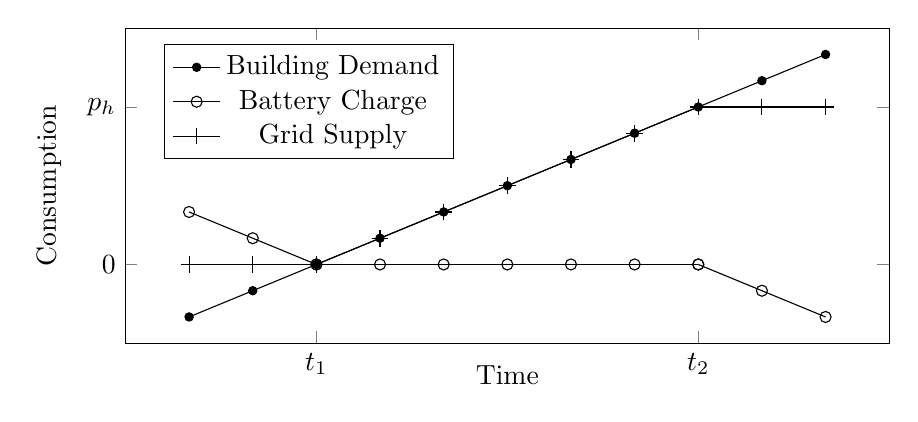
\begin{tikzpicture}

\begin{axis}[
width=0.8\columnwidth,height=4cm,scale only axis,
axis line style={-}, xtick style={-}, ytick style={-},
xlabel=Time,
ylabel=Consumption,
every axis y label/.style={at={(-0.1,0.5)},rotate=90,anchor=center}, 
every axis x label/.style={at={(0.5,-0.1)},anchor=center}, 
%grid=both, grid style={style=densely dotted},
xtick={2,8},
xticklabels={$t_1$,$t_2$},
ytick={0,6},
yticklabels={$0$,$p_h$},
legend style={at={(0.05,0.95)},anchor=north west}
] 

% Draw the Demand-Supply curve
\addplot[-,mark=*,mark size=1.5] expression[domain=0:10,samples=11] {x-2};
\addlegendentry{Building Demand} 

% Draw the Battery curve
\addplot[-,mark=o,mark size=2] expression[forget plot,domain=0:2,samples=3] {2-x}; 
\addplot[-,mark=o,mark size=2] expression[forget plot,domain=2:8,samples=7] {0}; 
\addplot[-,mark=o,mark size=2] expression[domain=8:10,samples=3] {8-x}; 
\addlegendentry{Battery Charge} 

% Draw the Grid supply curve
\addplot[-,mark=+,mark size=3] expression[forget plot,domain=0:2,samples=3] {0}; 
\addplot[-,mark=+,mark size=3] expression[forget plot,domain=2:8,samples=7] {x-2}; 
\addplot[-,mark=+,mark size=3] expression[domain=8:10,samples=3] {6}; 
\addlegendentry{Grid Supply} 
\end{axis} 
\end{tikzpicture} 

\end{center}
\caption{Use case scenario for the battery system during a $10$ hour period. The aim is to maintain grid consumption within the range $[0:6]$ units. Building Demand is the sum of individual loads and renewable generation and may therefore fall outside this range. By suitably ordering the charge or discharge of the battery system (Battery Charge signal), the net consumption (Grid Consumption signal) of the system may be maintained within range.}
\label{fig:usecase}
\end{figure}


\begin{figure}[ht]
\begin{center}
%!TEX root = ../aamas11storage.tex
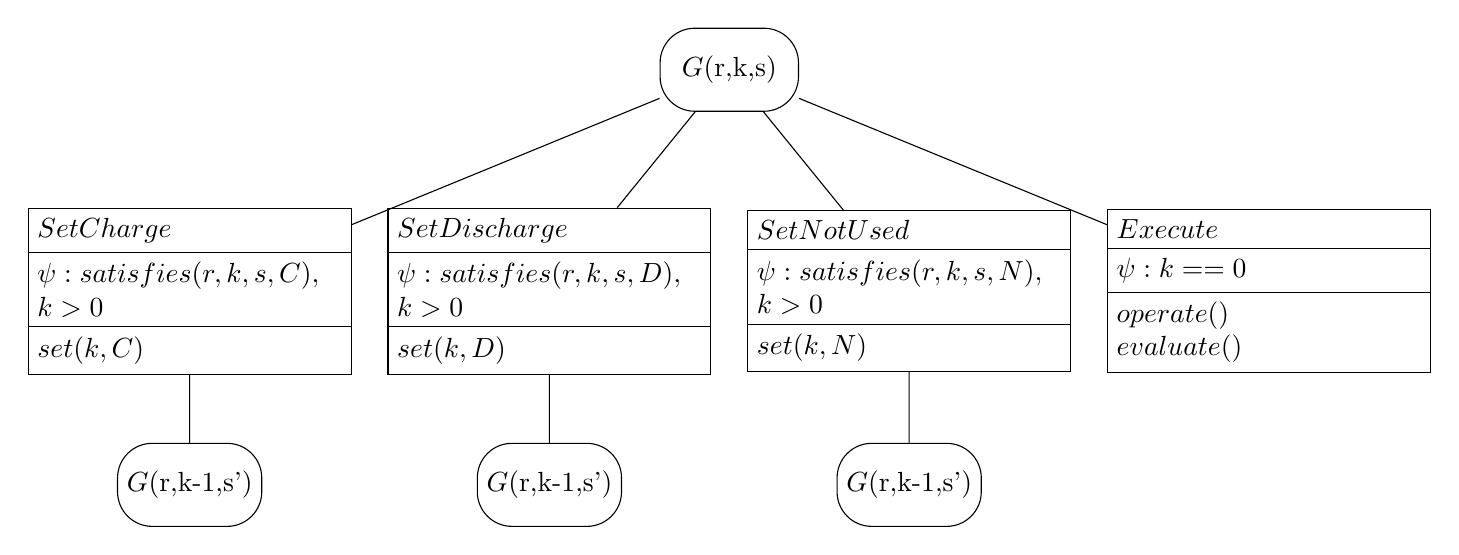
\begin{tikzpicture} [level distance=8.0em]
\tikzstyle{planbox}=[draw,text width=11.0em,rectangle split,rectangle split parts=3]
\tikzstyle{goalbox}=[draw,rounded corners=1.25em,minimum height=3em,minimum width=5em]

	
\tikzstyle{level 1}=[sibling distance=13.0em] 
\tikzstyle{level 2}=[level distance=7.0em] 

\node[goalbox,solid] {$G($r,k,s$)$}
	child {node[planbox] {$SetCharge$ 
			\nodepart{second} $\psi:satisfies(r,k,s,C),$\\$k>0$
			\nodepart{third} $set(k,C)$
		}
		child {node[goalbox] {$G($r,k-1,s'$)$}}
	}
	child {node[planbox] {$SetDischarge$ \nodepart{second}
			\nodepart{second} $\psi:satisfies(r,k,s,D),$\\$k>0$
			\nodepart{third} $set(k,D)$
		}
		child {node[goalbox] {$G($r,k-1,s'$)$}}
	}
	child {node[planbox] {$SetNotUsed$ \nodepart{second}
			\nodepart{second} $\psi:satisfies(r,k,s,N),$\\$k>0$
			\nodepart{third} $set(k,N)$
		}
		child {node[goalbox] {$G($r,k-1,s'$)$}}
	}
	child {node[planbox] {$Execute$ 
			\nodepart{second} $\psi:k==0$
			\nodepart{third} $operate()$ \\$evaluate()$
		}
	}
;

\end{tikzpicture}



\end{center}
\caption{Goal-plan hierarchy for the battery system with $k$ modules.}
\label{fig:gptree}
\end{figure}

Consider the example scenario of a smart office building that consists of a set of individual loads (appliances in the building), some renewable generators (solar panels on the roof and a local wind turbine), and a modular battery system. The building is connected to the main grid, and the economics govern that the grid power consumption of the building be maintained within the range $[0:6]$. Since there is little control over the demand in the building and certainly no control over the renewable generation, then for some period in the day it is possible that the power consumption of the building will fall outside this range. For instance, if the renewable generation is higher than the demand, then the consumption will be negative. Similarly, if the demand is higher than the renewable generation then the building consumption may rise above $P$. In Figure \ref{fig:usecase} the Building Demand curve shows the sum of consumption and generation in the building for a $10$ hour window some given day.

While there is little control over the consumption and generation in the building (Building Demand), we do have full control over how the battery system is used. So for instance, by suitably ordering the battery system to charge (act as a load) or discharge (act as a generator) at determined rates throughout the period we may influence the net demand in the building. Figure \ref{fig:usecase} shows how the appropriate battery response (Battery Charge curve) added to the building consumption and generation (Building Demand curve) ensures that the power drawn from the grid (Grid Consumption) is maintained within the desired range.

\section{Approach}

The battery system consists of a number of internal modules that may all have individual constraints. Moreover, the charge/discharge characteristics of the modules may change over time. As such, it is desirable that the battery control algorithm be able to adapt to these changes over time. Figure \ref{fig:gptree} shows a possible learning BDI agent controller for a battery system with $k$ modules. 

The top level goal $G(k,s)$ is posted by the system at the beginning of each period of deliberation. The controller then responds by operating the battery modules for that period in a suitable configuration that resolves the goal. The parameter $k$ is initially set to the number of modules in the system\footnote{Note that the battery design may contain more internal modules than the advertised number to provide for a operational buffer. In this case the parameter $k$ should reflect this actual count.}.  The parameter $s$ specifies the desired response from the system and lies in the normalised range $[-1.0:+1.0]$ where $-1.0$ indicates a maximum discharge rate and $+1.0$ indicates a maximum charge rate.

The resolution of the battery system determines how closely it can match the desired response and depends on the number of modules $n$. For simplicity, we will assume homogeneous capacity of the modules (but with possibly different chemical properties and constraints), such that each module has a capacity $c$ and $c*n=1.0$. Each internal module in turn may be in one of three states: charging (i.e $+c$), discharging (i.e. $-c$) or not in use (i.e. $0$). The sum of these values gives the net response of the system. In other words, the response of the battery system may be adjusted in multiples of $c$.

The BDI controller works by recursively setting the operational state of each module in the system using the $Set*$ plans, and then finally running the selected configuration for one period and evaluating the result using the $Execute$ plan. The execution therefore always consists of the selection of $k$ high level $Set*$ plans followed by the $Execute$ leaf plan. Using the BDI learning framework from \cite{Singh:RAS10} the pass/fail result is then recorded in the chain of active $Set*$ plans. By training over the outcomes of each plan selection in each situation, the system over time learns correct plan selection at each recursive level for the set of possible top-level requests.


Each plan in the goal-plan hierarchy is further explained below:

$SetCharge$: Plan to set the operational state of module $k$ to {\em Charge} for this period. The plan first checks that the internal constraints of module $k>0$ will not be violated by this operation. If a violation is expected, then the plan is aborted, otherwise the state is updated and Goal $G$ reposted for module $k-1$.

$SetDischarge$: Plan to set the operational state of module $k$ to {\em Discharge} for this period. The plan first checks that the internal constraints of module $k>0$ will not be violated by this operation. If a violation is expected, then the plan is aborted, otherwise the state is updated and Goal $G$ reposted for module $k-1$.

$SetNotUsed$: Plan to set the operational state of module $k$ to {\em NotUsed} for this period. This means that the module will remain disconnected from use for this period. The plan first checks that the internal constraints of module $k>0$ will not be violated by this operation. If a violation is expected, then the plan is aborted, otherwise the state is updated and the Goal $G$ reposted for module $k-1$.

$Execute$: The leaf plan that actually performs the operations on the battery modules. The plan operates only when $k=0$ which implies that all modules have been configured. The battery modules are then operated for this period according to their assigned states. At the end of the period, the plan will evaluate the battery response against the goal and determine the $Pass$ or $Fail$ status. Normally, a pass would mean that the actual battery response was within tolerance of the desired response. 


The $Set*$ plans in the hierarchy may fail when selected if the constraints for module $k$ are violated for that period. For instance, plan $SetCharge$ might fail because module $k$ is only allowed to change charge directions once every four periods say, and charging it in this period will violate that constraint. Similarly, plan $SetDischarge$ might fail because the module may have critically low charge and further discharge for a full period is not possible. Finally, plan $SetNotUsed$ might fail because the module has a requirement to be fully discharged once every day, and disconnecting it in this period will violate that constraint. 

Since violation checks are performed prior to taking any action, then BDI failure recovery may be performed to select a different $Set*$ plan until all internal constraints are satisfied prior to execution. Note that failure recovery is not allowed for the $Execute$ plan because it runs for a full period and that is the limit for the decision making. In other words, only one try is allowed per period. So functionally, the $Execute$ plan must always succeed, even though the evaluation against the goal (for learning purposes) may differ.

Finally, the system only learns a response to the immediate request i.e. how to resolve the top level goal. It does not learn any temporal relationship in the sequence of top level goals. For instance, the input signal may have some diurnal pattern, however the proposed system does not attempt to learn this pattern.





\section{Implementation Notes}

The system is (purposely) similar in design to the Towers of Hanoi problem of \cite{Singh:RAS10}. In some respects, it is simpler because the solutions are always at recursive depth $k$. Moreover, the non-leaf $Set*$ plans do not have side-effects when they fail and leave the initial state unaltered. Finally, a solution always consists of a single $Execute$ action whereas in the Hanoi problem it consists of possibly several $Move$ actions\footnote{One point of difference is that this is not a universal library where a solution can always be found. For some requests, no solution will be possible given the internal state of the modules.}.

Nonetheless, the problem captures a real world problem where it is not straightforward to hand-craft a functional hierarchy and where learning is justified. We do not have a solution to begin with. Then, the size of the problem is still significant - the flow battery in CSIRO Newcastle has $10$ internal modules, so with three possible module states that represents $3^{10}=59049$ possible configurations for a given request. Finally, it offers a realistic scenario for re-learning a solution due to significant changes in the environment. For instance, if an internal module were to fail and had to be replaced, then prior learning may no longer work effectively, and the system will have to adjust and re-learn it's response based on the new characteristics of the updated module.

%%
\begin{thebibliography}{10}

\bibitem{Airiau:IJAT09}
S.~Airiau, L.~Padgham, S.~Sardina, and S.~Sen.
\newblock Enhancing Adaptation in {BDI} Agents Using Learning Techniques.
\newblock In {\em International Journal of Agent Technologies and Systems},
2009.

\bibitem{Singh:AAMAS10}
D.~Singh, S.~Sardina, L.~Padgham, S.~Airiau.
\newblock Learning Context Conditions for {BDI} Plan Selection.
\newblock In {\em Proceedings of Autonomous Agents and Multi-Agent Systems (AAMAS)}, 2010.

\bibitem{Singh:RAS10}
D.~Singh, S.~Sardina, L.~Padgham.
\newblock Extending BDI Plan Selection to Incorporate Learning from Experience.
\newblock Robotics and Autonomous Systems, 2010.


\end{thebibliography}

\end{document}